\documentclass[aspectratio=169]{beamer}
\usepackage[utf8]{inputenc}
\usepackage[T1]{fontenc}
\usepackage{ragged2e}
\usepackage{cite}
\usepackage{graphicx}
\usepackage{multimedia}
\usepackage{multirow}
\usepackage{hyperref}
\usepackage{xcolor}
\usepackage{color}
%\hypersetup{bookmarksopen=true, bookmarksopenlevel=1}


\title[Multi-echo fMRI for overt speech production ]{Multi-echo fMRI for overt speech production } 
\date{September, 2024 }
\author{Flores-Coronado M.A., Martin C. \& Caballero-Gaudes C. \vspace{1.4cm}

\includegraphics[width=0.5\textwidth]{images/BCBL_SPiN_copy}}


\usetheme{spin}
\begin{document}
\begin{frame}
\maketitle
\end{frame}



\begin{frame}{Overview}
	\begin{center}
		\begin{huge}
		Project phases
		\end{huge}
	\end{center}
	\begin{enumerate}
		\setlength\itemsep{3em}
		\item{Methods for \textit{fMRI speech production} (\textbf{Methods development}).}
		\item{\textit{Foreign sound learning}, a fMRI experiment (\textbf{Methods implementation}).}
	\end{enumerate}
\end{frame}

\begin{frame}
	\frametitle{Magnetic Resonance Imaging (MRI) --DEVELOPMENT--}
\begin{columns}
\column{.5\textwidth}
\begin{tiny}
	\begin{itemize}
		\item[]<1-3>{\color{red}{How does it work?}}
		\item[]<4>{\color{red}{Measument noise sources!}}
	\end{itemize}
\end{tiny}
	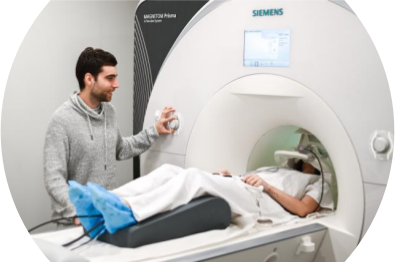
\includegraphics[width=.8\textwidth]{images/MRI.png} 
\column{.5\textwidth}
\includegraphics<1>[width=\textwidth]{images/spin0} 
\includegraphics<2>[width=\textwidth]{images/spin1} 
\includegraphics<3>[width=\textwidth]{images/spin2} 
\includegraphics<4>[width=\textwidth]{images/noiseSpeech} 
\end{columns}
%\begin{center}
%\begin{tiny}
%\cite{Barsalou2003, Barsalou2018,Kuhnke2020 ,Twomey2020}
%\end{tiny}
%\end{center}
\end{frame}

\begin{frame}{fMRI parameters \textit{Methods development}}
	\begin{columns}
		\column{.4\textwidth}
		\begin{center}
				\textbf{Problem}
		\end{center}
			\begin{tiny}
				\begin{itemize}
					\item[]<1>{What's the best to sample speech production with fMRI?}
					\item[]<2>{How do we clean noise originated in MRI machine?}
				\end{itemize}
				\end{tiny}
		\begin{center}
				\textbf{Work done}
		\end{center}
				\begin{flushleft}
			\begin{tiny}	
				\begin{itemize}
					\item[]<1>{Comparition of computer simulations with different methods}
					\item[]<2>{Development and comparison to reduce noise and improve signal measurement.}
				\end{itemize}

			\end{tiny}
		\end{flushleft}
\column{.6\textwidth}
		\begin{center}
			\includegraphics<1>[width=.6\textwidth]{images/complex_cm}
			\includegraphics<2-3>[width=\textwidth]{images/nordic_flow} 	
		\end{center}
	\end{columns}
\end{frame}


\begin{frame}{Speech denoising \textit{Methods development}}
	\begin{columns}
		\column{.4\textwidth}
		\begin{center}
				\textbf{Problem}
		\end{center}
		\begin{tiny}
			\begin{itemize}
				\item[]<1>{The more speech, the more artifacts.}
				\item[]<2>{Need to classify artifacts from signal.}
			\end{itemize}
		\end{tiny}
		\begin{center}
				\textbf{Work done}
		\end{center}
		\begin{tiny}
			\begin{itemize}
				\item[]<1>{Speech experiment (e.g., syllables, words, sentences).}
				\item[]<2>{Build signal classification algorithm (in course).}
			\end{itemize}
		\end{tiny}
		\column{.6\textwidth}
		\begin{center}
			\includegraphics<1>[width=.6\textwidth]{images/complex_cm}
			\includegraphics<2-3>[width=\textwidth]{images/nordic_flow} 	
		\end{center}
	\end{columns}
\end{frame}



\begin{frame}{Thanks}
\begin{center}
\includegraphics<1>[width=.9\paperwidth]{images/thanks}
\end{center}
\end{frame}

\bibliographystyle{apalike}
\bibliography{Library}




\end{document}
